Este capítulo apresenta os resultados obtidos a partir da metodologia descrita no Capítulo 3. Os dados são organizados em tabelas e gráficos para facilitar a análise e comparação com valores teóricos ou da literatura.

\section{Resultados Experimentais}

A Tabela~\ref{tab:resultados} apresenta os valores medidos para cada condição de ensaio, incluindo a incerteza associada.

\begin{table}[H]
\centering
\caption{Resultados dos ensaios de tração.}
\label{tab:resultados}
\begin{tabular}{lccc}
\toprule
Amostra & Tensão máxima (MPa) & Deformação (\%) & Módulo (GPa) \\
\midrule
A1 & $285 \pm 12$ & $18,2 \pm 0,8$ & $71,3 \pm 1,5$ \\
A2 & $291 \pm 10$ & $17,8 \pm 0,6$ & $72,1 \pm 1,2$ \\
A3 & $278 \pm 15$ & $19,1 \pm 1,0$ & $70,8 \pm 1,8$ \\
\midrule
Média & $285 \pm 7$ & $18,4 \pm 0,5$ & $71,4 \pm 0,9$ \\
\bottomrule
\end{tabular}
\end{table}

\section{Análise Gráfica}

A Figura~\ref{fig:resultados} compara os valores experimentais com os valores teóricos previstos pelo modelo.

\begin{figure}[H]
\centering
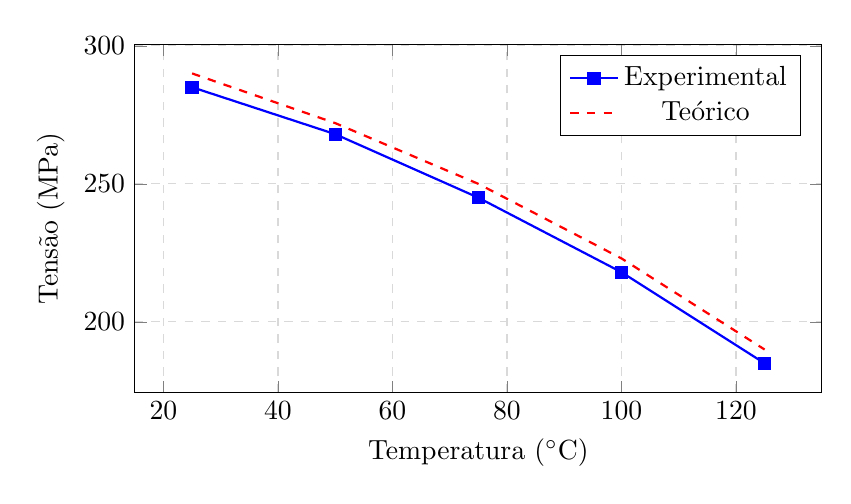
\begin{tikzpicture}
\begin{axis}[
    width=0.85\textwidth,
    height=6cm,
    xlabel={Temperatura ($^\circ$C)},
    ylabel={Tensão (MPa)},
    legend pos=north east,
    grid=major,
    grid style={dashed, gray!30},
]
\addplot[blue, mark=square*, thick] coordinates {
    (25, 285) (50, 268) (75, 245) (100, 218) (125, 185)
};
\addplot[red, dashed, thick] coordinates {
    (25, 290) (50, 272) (75, 250) (100, 223) (125, 190)
};
\legend{Experimental, Teórico}
\end{axis}
\end{tikzpicture}
\caption{Variação da tensão máxima com a temperatura.}
\label{fig:resultados}
\end{figure}

\section{Comparação com a Literatura}

A Tabela~\ref{tab:comparacao} compara os resultados obtidos com valores reportados na literatura.

\begin{table}[H]
\centering
\caption{Comparação com valores da literatura.}
\label{tab:comparacao}
\begin{tabular}{lccc}
\toprule
Fonte & Tensão (MPa) & Deformação (\%) & Condições \\
\midrule
Este trabalho & $285 \pm 7$ & $18,4 \pm 0,5$ & 25$^\circ$C, 1 mm/min \\
\textcite{Degarmo2003} & $275$ & $17,0$ & 23$^\circ$C, 2 mm/min \\
\textcite{Howard1971} & $290$ & $19,5$ & 25$^\circ$C, 1 mm/min \\
\bottomrule
\end{tabular}
\end{table}

Os valores obtidos estão dentro da faixa esperada, com diferença inferior a 5\% em relação à literatura. A pequena variação pode ser atribuída a diferenças na composição do material e nas condições de ensaio.

\section{Exemplo de Tabela Longa}

A Tabela~\ref{tab:especificacoes} demonstra o uso de tabelas longas que continuam em múltiplas páginas.

\begin{longtable}{p{0.35\textwidth} p{0.55\textwidth}}
\caption{Especificações técnicas do espectro-radiômetro SR-5000.}
\label{tab:especificacoes} \\

\toprule
\textbf{Especificação} & \textbf{Descrição} \\
\midrule
\endfirsthead

% Cabeçalho das páginas seguintes
\multicolumn{2}{c}{\tablename\ \thetable{} -- (Continuação da Tabela \thetable)} \\
\midrule
\textbf{Especificação} & \textbf{Descrição} \\
\midrule
\endhead

% Rodapé das páginas intermediárias
\midrule
\multicolumn{2}{r}{\textit{(Continua na próxima página)}} \\
\endfoot

% Rodapé da última página
\bottomrule
\endlastfoot

% Conteúdo da tabela
Óptica & Lente telescópica totalmente reflexiva, com 5 polegadas de diâmetro (f/n$^{\text{o}}$ = 4) \\
Alcance do foco & De 2,5 metros até o infinito \\
Faixa espectral & 0,24 a 14,3 µm \\
Resolução espectral segmentada & Aproximadamente 2\% do comprimento de onda \\
Campo de visão (FOV) & 0,3 mrad a 6 mrad \\
Taxas de varredura & Padrão: até 10 varreduras por segundo \\
Alinhamento com o alvo & Sem paralaxe na linha de visão por meio do conjunto óptico \\
Uniformidade do FOV & $\pm$10\% (tipicamente $\pm$5\%) \\
Tipos de detector & Intercambiáveis pelo usuário (inclusive em campo), sem necessidade de realinhamento \\
Corpo negro interno & Monitoramento com precisão melhor que 0,1 °C à temperatura ambiente \\
Frequência de \textit{chopping} & 100 a 1800 Hz \\
Desempenho de ruído & Dependente do comprimento de onda e do detector \\
Linearidade & Melhor que 0,1\% da faixa total \\
Estabilidade de ganho & Melhor que 0,05\% por hora após aquecimento \\
Alimentação elétrica & 110/220 VAC, 50/60 Hz, 150 W máximo \\
Temperatura de operação & 10 °C a 40 °C \\
Umidade de operação & 10\% a 90\% (sem condensação) \\
Dimensões & 450 $\times$ 320 $\times$ 280 mm \\
Peso & 18 kg (sem acessórios) \\
Interface de comunicação & RS-232, USB 2.0, Ethernet \\
Software de controle & Compatível com Windows 10/11 \\
Certificações & CE, FCC, RoHS \\
Garantia & 2 anos para peças e mão de obra \\

\end{longtable}
